\documentclass[draft]{article}
\usepackage{tikz}

\title{Mathematics for physics}
\author{@t-34400}

\begin{document}
\maketitle
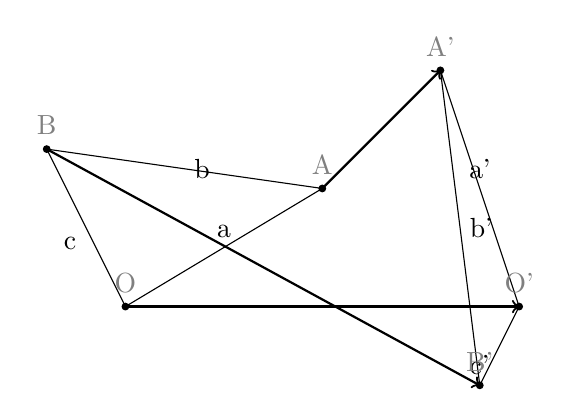
\begin{tikzpicture}
  \coordinate (O) at (0,0);
  \coordinate (A) at (2.5,1.5);
  \coordinate (B) at (-1,2);
  \coordinate (O') at (5,0);
  \coordinate (A') at (4,3);
  \coordinate (B') at (4.5,-1);

  \draw (O) -- node[above]{a} (A) -- node[right]{b} (B) -- node[below left]{c} cycle;
  \draw (O') -- node[above]{a'} (A') -- node[right]{b'} (B') -- node[below left]{c'} cycle;
  \foreach \p in {O,A,B,O',A',B'}
    \node[fill,circle,inner sep=1pt,label=\textcolor{gray}{\p}] at (\p) {};
  \draw[->,thick] (O) -- (O');
  \draw[->,thick] (A) -- (A');
  \draw[->,thick] (B) -- (B');
\end{tikzpicture}
\end{document}